\documentclass[tikz,border=7pt]{standalone}
\usetikzlibrary{calc}
\begin{document}
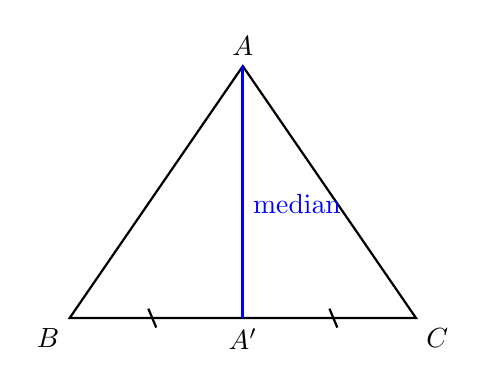
\begin{tikzpicture}[line width=.8pt]
\coordinate (A) at (0,3.2); \coordinate (B) at (-2.2,0); \coordinate (C) at (2.2,0); \coordinate (M) at (0,0);
\draw (A)--(B)--(C)--cycle; \draw[blue,very thick] (A)--(M);
\draw (-1.2,.12)--(-1.1,-.12); \draw (1.1,.12)--(1.2,-.12);
\node[above] at (A) {$A$}; \node[below left] at (B) {$B$}; \node[below right] at (C) {$C$}; \node[below] at (M) {$A'$};
\node[blue,right] at (0,1.45) {median};
\end{tikzpicture}
\end{document}
